\chapter{Begriffe im Maschinellen Lernen}
\label{cha:Begriffe}

Diese Erklärung der Begriffe und Elemente verfolgt zwei Ziele.
Zum Einen stellt dies Grundlage des gesamten Themas dar und soll für Interessierte, die nicht so vertraut sind, eine Einführung in die Thematik bieten. 
Und zum Anderen werden viele dieser Begriffe erläutert, welche noch häufig zum Einsatz kommen (u.A. Neuron, Aktivierungsfunktion, …).

\section{Data Science}

Data Science wird generell als die Extraktion von Wissen aus Daten bezeichnet. 
Dabei werden die Fachbereiche Statistik und Mathematik, Informatik und Machine Learning sowie einige weitere, mit diesem Begriff zusammengefasst. 
Das Gebiet für sich wird auch als Berufstätigkeit bezeichnet, wobei meist spezialisierte Formen für die Berufsbezeichnung verwendet werden. \newline

\noindent 
Damit Wissen aus Daten überhaupt extrahiert werden kann, muss ein ganzer Prozess durchlaufen werden. 
Dieser beginnt mit dem Zusammentragen von Rohdaten aus der Realität, welche zu diesem Zeitpunkt noch keinen Zusammenhang offenbaren. 
Im zweiten Prozessschritt werden diese Daten meist umgebaut und neu sortiert, wobei dieser Schritt nicht immer erforderlich ist. 
Auf die zurecht gelegten Daten besteht nun die Möglichkeit Modelle, Algorithmen sowie weitere Extraktionen durchzuführen. 
Die erneut extrahierten Daten werden in weiterer Folge als Ausgangsdaten verwendet. 
Auf diese Daten ausgeführte Modelle und Algorithmen liefern Ergebnisse, die visuell dargestellt für eine größer Gruppe von Personen geeignet sind. 
Aus diesem gelernten Wissen besteht zusätzlich die Möglichkeit dieses zum Generieren von neuen Daten zu verwenden und neue Modelle zu entwickeln, die zum Beispiel Vorgänge in der Natur noch akkurater widerspiegeln.

\section{Machine Intelligence}

Machine Intelligence ist ein Begriff, der noch nicht definiert worden ist, aber schon Verwendung findet. 
Einige namhafte Unternehmen wie Google Inc. und Microsoft Corporation bieten jeweils unterschiedliche Definitionen oder Beschreibungen. 
Die Definitionen dieser Firmen weichten nur unwesentlich voneinander ab.
%Dieser wird aber von allen ähnlich beschrieben und definiert.
Dieser Begriff wird als Überbegriff über das gesamte Gebiet mit Machine Learning, Künstlicher Intelligenz, Konversationsintelligenz und alle Themen die in näherer Beziehung dazu stehen verwendet. 

\section{Machine Learning}
\label{sec:Machine Learning}

Machine Learning definiert eine große Anzahl an Theorien und Umsetzungen von nicht explizit programmierten Abläufen. 
Diese wurden aus Studien in den Bereichen der Mustererkennung und der rechnerischen Lerntheorie mit Künstlicher Intelligenz teilweise entwickelt. 
Dieses Gebiet umfasste im Jahr 2016 aber sehr viel mehr. 
So existieren zusätzliche Ansätze aus dem Bereich der Biologie wie zum Beispiel Neuronale Netzwerke, die dem Gehirn nachempfunden sind und genetische Algorithmen, die der Weiterentwicklung eines Lebewesens ähneln. 
Ein ganz anderer Zugang wurde in der Sowjetunion verfolgt, mit sogenannten 'Support Vektor Machines', bei welchem man einen rein mathematischen Ansatz anstrebt. \cite{lampropoulos2015machine}

\section{Neuronale Netzwerke}

Neuronale Netzwerke sind seit einigen Jahren auch bekannt unter dem Begriff 'Deep Learning'. \newline

\noindent 
Die Theorie und die ersten Grundlagen wurden im Jahre 1943 von Warrn McCulloch und Walter Pitts geschaffen, die ein Modell entwickelten, jedoch nicht die technischen Möglichkeiten hatten dieses umzusetzen.
Dieses %basierte auf Mathematik und Algorithmen und 
führte zur 'Threshold Logik', welche bestimmt ab wann etwas weitergegeben wird und wie stark ausgeprägt. \cite{rojas2013neural}
%\textbf{TODO: beschreiben}
Durch den Grundstein des 'Backpropagation'-Algorithmus im Jahre 1975 ist es möglich, Netzwerke mit mehr als drei Ebenen zu trainieren. 
Neuronale Netzwerke bestehen aus Neuronen, die miteinander verbunden sind und gemeinsam ein Netzwerk ergeben. \cite{AI3} %, welches dem Gehirn gleicht. %nachempfunden ist. 
%Die Verbindungen sind nicht fest vorgegeben, sondern können auch zum Beispiel Schleifen bilden.}

%TODO: you can do anything with it, if it can be designed as a function


\section{Neuron}
\label{sec:Neuron}

%Abbildung ( Aufbau eines Neurons ) - TikZ Grafik \\
\begin{figure}
\centering

\begin{tikzpicture}
	
	\node[neuron] (a) {};
	\node[neuron,below=of a] (b) {};
	\node[neuron,below=of b] (c) {};
	
	\node[neuron,right=of b] (root) {$\phi(\sum)$};
	
	\node[right=of root] (out) {};

	\node[group,fit={(a) (b) (c)}] (gr1) {};
	\draw[conn] (a) -- (root);
	\draw[conn] (b) -- (root);
	\draw[conn] (c) -- (root);
	\draw[conn] (root) -- (out);

\end{tikzpicture}

	\caption{Neuron mit Eingang, Kernfunktion, Aktivierungsfunktion}
	\label{fig:Neuron}
\end{figure}

%\noindent 
Ein Neuron wurde einer Nervenzelle in einem Gehirn nachempfunden mit den folgenden Bestandteilen:
\paragraph{Informationseingangsstrom} ist der Dateneingang, wobei ein Neuron ein bis theoretisch beliebig viele solcher Eingänge haben kann. 
Dies hängt von der jeweiligen Architektur des Netzwerks ab.

\paragraph{Informationsgewichtung} bezeichnet die Gewichtung mit der der Eingangsstrom gewertet wird. 
%Dies wird Gewichtung genannt. 
So wird ein Informationseingangsstrom mehr oder weniger berücksichtigt. 
Diese Gewichtung wird durch den Backpropagation-Algorithmus angepasst und nachjustiert.

\paragraph{Kernfunktion} bewirkt das Verarbeiten der gewichteten Informationseingänge. 
Im einfachsten Fall werden alle Werte aufsummiert. 
Es wäre aber möglich, jegliche Berechnung hier einfließen zu lassen, welche mehrere Werte verwendet und daraus einen neuen Wert berechnet.

\paragraph{Aktivierungsfunktion} berechnet den Ausgang eines Neurons. 
Dabei wird eine weitere Funktion auf das im Kern berechnete Ergebnis ausgeführt und führt dazu, dass ein Ergebnis noch stärker ausgeprägt weitergegeben wird oder minimiert wird, beziehungsweise in einen Wertebereich eingepasst wird. 
Diese Aktivierungsfunktion ist meist die Sigmoid-Funktion oder eine lineare Funktion, welcher in der Abbildung \ref{fig:Aktivierungsfunktion} zu erkennen sind.

%\textit{Grafiken zu Sigmoid und lineare}
%Wobei in den vergangen Jahren die Linearen-Funktionen häufiger zum Einsatz kommen.
%\\
\begin{figure}[ht!]
\centering
%\begin{minipage}{0.7\linewidth}
\subfloat{
\resizebox {0.5\linewidth} {5cm} {
	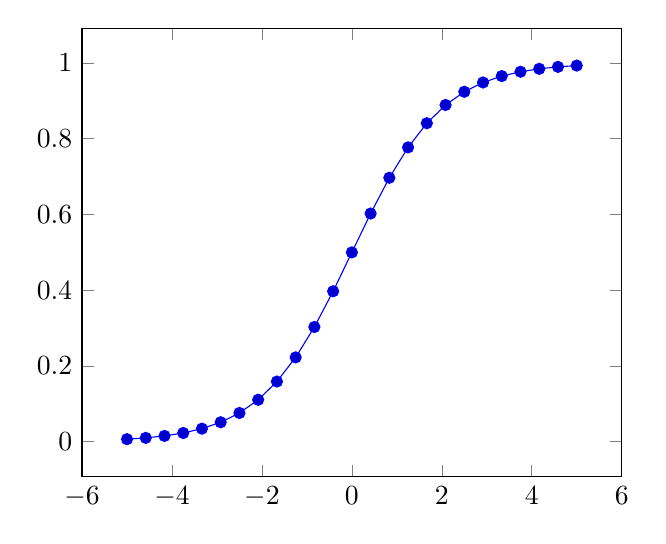
\begin{tikzpicture}
	\begin{axis}

		\addplot expression { 1/(1+exp(-x) };

	\end{axis}
	\end{tikzpicture}
}
%\end{minipage}
}
\subfloat{
%\begin{minipage}{0.7\linewidth}
\resizebox {0.5\linewidth} {5cm} {
	\begin{tikzpicture}
	\begin{axis} [xmin=-1, xmax=1]

		\addplot expression { x };

	\end{axis}
	\end{tikzpicture}
}
%\end{minipage}
}
	\caption{Basisaktivierungsfunktionen: (l) eine Sigmoid-Funktion, (r) eine lineare Funktion}
	\label{fig:Aktivierungsfunktion}
\end{figure}

\noindent 
Die einfachste Repräsentation eines Neurons lässt sich mathematisch folgendermaßen darstellen.
Im Kern wird eine Summenberechnung durchgeführt. 
Dabei werden die Eingangswerte und deren Gewichtung miteinander multipliziert, sowie diese Ergebnisse aufsummiert.
Der griechische Buchstabe $\phi$ (phi) steht für die Aktivierungsfunktion des Neurons und stellt damit die Ausgabe des Neurons dar.
\begin{equation}
	f(x, w) := \phi ( \sum\limits_{i}{w_i * x_i})
	\label{eq:Aktivierungsfunktion}
\end{equation}

%\section{Bias Neuron}
%\label{sec:Bias Neuron}

\paragraph{Bias Neuron} 
\label{sec:Bias Neuron}

definiert einen Spezialfall eines Neurons, welches keine Dateneingänge somit auch keine Gewichtung hat und keine Berechnung im Kern durchführt. 
Dieses liefert nur einen konstanten Wert, wie zum Beispiel eine $1$. 
Durch die konstante Auslieferung wird auch die Aktivierungsfunktion überflüssig. 
Das Bias Neuron stellt somit einen stetigen Wert für das Netzwerk dar, beziehungsweise für die darauffolgende Ebene.

\section{Ebenen/Layer}
\label{sec:Layer}

Ebenen sind Zusammenschlüsse von Neuronen, welche sich auf der selben Stufe befinden. 
Diese Neuronen sind aber nicht miteinander verbunden, sondern bekommen Daten aus der Ebene davor und geben diese an die darauffolgende Ebene weiter. 
Dieser Typ wird \textbf{Hiddenlayer} bezeichnet. 
Jedes Netzwerk benötigt zusätzlich zwei weitere Ausprägungen an Ebenen. 
Diese sind:

%\textit{\textbf{TODO}}
\paragraph{Inputlayer} stellt den Übergang zwischen der Welt außerhalb des Neuronalen Netzwerks und dem Netzwerk dar.
Diese Ebene nimmt die Daten ohne Gewichtung auf und gibt sie an die darauffolgende Ebene weiter. 
%In gewisser Weise stellt sie einen Übergang zwischen der Außenwelt und des Neuronalen Netzwerkes dar.

%\textit{\textbf{TODO}}
\paragraph{Outputlayer} befindet sich am Ende eines Netzwerkes. 
Dieser Layer hat die Aufgabe, die Daten nach außen weiterzugeben, oder an das darauffolgende Netzwerk. 
Hierbei werden die Informationen meist nur mehr für die Ausgabe aufbereitet. 
In manchen Netzwerken existieren keine Outputlayer in diesem Sinne, sondern ein Layer, der als Hiddenlayer und Outputlayer fungiert. 
Dies ist der Fall, wenn nur zwei Layer sich im Netzwerk befinden und einer davon vom Inputlayer eingenommen wird.
%So wird zum Beispiel die Wahrscheinlichkeit für jeden Ausgang berechnet.
\\

%Abbildung ( Aufbau eines Einfachen FeedForward NN) - TikZ Grafik
\begin{figure}
\centering

\begin{tikzpicture}

	\node[neuron] (in) {I};

	\node[neuron,right=of in] (1a) {N};
	\node[neuron,below=of 1a] (1b) {N};
	\node[io,below=of 1b] (b1) {B};
	
	\node[group,fit={(1a) (1b) (b1)},right=of in] (gr1) {};
	
	\node[neuron,right=of 1a] (2a) {N};
	\node[neuron,below=of 2a] (2b) {N};
	\node[io,below=of 2b] (b2) {B};
	
	\node[group,fit={(2a) (2b) (b2)},right=of 1a] (gr2) {};
	
	\node[neuron,right=of 2a] (3a) {N};
	\node[neuron,below=of 3a] (3b) {N};
	\node[io,below=of 3b] (b3) {B};
	
	\node[group,fit={(3a) (3b) (b3)},right=of 2a] (gr3) {};
	
	\node[neuron,right=of 3b] (out) {O};
	
	\draw[conn] (in) -- (1a);
	\draw[conn] (in) -- (1b);

	\draw[conn] (1a) -- (2a);
	\draw[conn] (1a) -- (2b);
	
	\draw[conn] (1b) -- (2a);
	\draw[conn] (1b) -- (2b);

	\draw[conn] (b1) -- (2a);
	\draw[conn] (b1) -- (2b);
	
	
	\draw[conn] (2a) -- (3a);
	\draw[conn] (2a) -- (3b);
	
	\draw[conn] (2b) -- (3a);
	\draw[conn] (2b) -- (3b);

	\draw[conn] (b2) -- (3a);
	\draw[conn] (b2) -- (3b);
	
	
	\draw[conn] (3a) -- (out);
	\draw[conn] (3a) -- (out);
	
	\draw[conn] (3b) -- (out);
	\draw[conn] (3b) -- (out);

	\draw[conn] (b3) -- (out);
	\draw[conn] (b3) -- (out);

\end{tikzpicture}

	\caption{Einfaches Neuronales FeedFordward Netzwerk}
	\label{fig:SimpleFeedForwardNetwork}
\end{figure}

\section{Informationen Merken und Wiedererkennung}

Durch das Anpassen der Gewichtungen bei jedem Dateneingangsstrom mit Hilfe des Backpropagation-Algorithmus ist es möglich, Zustände zu speichern und diese auch zu merken. 
Sollte ein ähnlicher Dateneingang stattfinden, wo zuvor schon einer einmal vorhanden war, dann sollte dieser ähnlich behandelt werden.
%Dies führt dazu, sollte ein ähnlicher Dateneingang stattfinden, wo zuvor schon ein ähnlicher in einem Trainingszyklus vorhanden war, dies erkannt wird. %\textit{dieser ähnliche erkannt wird. \textbf{TODO}} 
Dieser kann möglicherweise zu derselben Kategorie gehören, wie der zuvor schon bekannt gemachte und gelernte Dateneingang.

\section{Konvergieren im Maschinellen Lernen}
\label{sec:Konvergieren}

Konvergieren im Maschinellen Lernen bezeichnet das Minimieren der Fehlerquote gegen $0$.
Die Fehlerquote wird dabei als Error bezeichnet und ist ausschlaggebend für den Lernprozess.
Eine Error von $0$ würde bedeuten, dass das Netzwerk keinen Fehler machen würde.
Für die Feststellung des Fehlers gibt es diverse Funktionen wie zum Beispiel die 'Mean-Square-Error'-Methode.

\section{Backpropagation}
\label{sec:Backpropagation}

%TODO: relative genauer Algorithmus mit Aufgabe
Bis zum Jahre 1986 gab es keine automatisierte Möglichkeit, die Gewichtungen in einem Netzwerk automatisch anzupassen.
In diesem Jahre entwickelten Rumelhart, Hinton \& Williams eine mögliche Lösung, welche sehr ähnlich zu anderen Ansätzen von früher war (Werbos, 1974; Parker, 1985; Cun, 1985).
Die zentrale Idee in ihrer Lösung liegt darin, die Abweichung des produzierten Ergebnisses zum wirklichen erwarteten Ergebnis zu bestimmen. 
Aufgrund dieses Fehlers lassen sich im Anschluss die Gewichtungen im Netzwerk vom Ende zum Anfang nachjustieren. 
Diese Technik ermöglichte damit tiefe Netzwerke zu konstruieren und auch zu trainieren.

\paragraph{Lernrate} skaliert die Steigung des Lernprozesses, mit der Auswirkung ob schneller oder langsamer gelernt wird.
Eine Lernrate unter $0$ würde die Lerngeschwindigkeit stark verlangsamen. 
Ein Wert über $1$ würde eine hohe Lerngeschwindigkeit zur Folge haben. 
Eine zu hohe Rate würde nicht zum Konvergieren \ref{sec:Konvergieren} führen, sondern zum Springen.

\paragraph{Momentum} stellt wie die Lernrate eine Skalierung des Lernprozesses dar.
Dabei werden mit dem definierten Faktor die früheren Gewichtsupdates berücksichtigt. 
Dies führt dazu, dass lokale Tiefpunkte überwunden werden können und das System doch zum globalen Tiefpunkt konvergiert.

%\textit{\textbf{TODO}}
\section{Allgemeine Probleme}
\label{sec:AllgeProb}

Nach dem aktuellen Stand der Dinge können Neuronale Netzwerke nicht jede Frage dieser Welt beantworten.
Das Entwickeln eines neuen Netzwerks ist eine sehr schwierige und eine lang andauernde Aufgabe. 
Dabei können Fehler auftreten, welche natürlicher Natur sein können, aber auch durch den Entwickler verursacht sein können. \\

%Neuronale Netzwerke sind nicht Fehler- und Problemlos und können nicht jegliche Fragen in dem Themengebiet lösen. 
%Es existieren bekannte Probleme für die es Lösungen oder Lösungsansätze gibt. 
%Es gibt aber auch noch genügend andere Probleme, welche noch nicht festgestellt wurden oder als solche noch nicht erkannt worden sind. 

\noindent
Diese Arbeit wird auf die bekanntesten Probleme eingehen und auch Lösungen oder mögliche Lösungsansätze beinhalten. 

%\subsection{Overfitting}

\paragraph{Overfitting} bezeichnet ein Problem, welches nicht nur Machine Learning betrifft, sondern auch Menschen und andere Lebewesen. 
Ein Student lernt zum Beispiel auf eine Prüfung und ist im Besitz einer Klausur aus einem Vorjahr. 
Nach öfterem Durchspielen der Fragen und sich selbst testen, befindet er sich in der Lage diese Klausur mit einer sehr hohen Wahrscheinlichkeit zu bestehen. 
Dabei hat sich die Klausur in seinem Gehirn eingeprägt, aber nicht das Stoffgebiet zu welchem er eine Klausur schreiben muss. 
Das Problem wird als Overfitting bezeichnet und beschreibt, dass etwas gemerkt wurde, aber nicht gelernt worden ist und somit eine Abwandlung von Informationen nicht wiedererkannt wird.

%\subsection{Daten & Datensätze}

%TODO: jeder Datensatz ist unterschiedlich -> neue Daten = neues Netzwerk
\paragraph{Daten} die zum Trainieren von Netzwerken verwendet werden, stellen selbst Probleme dar.
% Ein weiteres Problem stellen die Daten und Datensätze dar, welche zum Trainieren des Netzwerkes verwendet werden.
Eine zu geringe Menge an Daten stellt den Entwickler vor das Problem, dass er für diese Daten ein akkurates Netzwerk entwickeln kann.
Dieses Netzwerk würde aber möglicherweise nicht die gewünschten Resultate liefern, da die zur Verfügung gestellten Daten nur einen kleinen Teil des Gesamten repräsentieren.
Zusätzlich kann es sein, dass die zur Verfügung gestellten Daten selbst nicht vollständig sind und somit wieder nur ein Subset verwendet werden kann.

\paragraph{Datensätze} können ähnlich sein zu anderen, sind aber trotzdem wieder einzigartig. 
Dies bedeutet, dass ein Netzwerk, welches für eine Problemstellung entwickelt und trainiert wurde, nicht eins zu eins übernommen werden kann.
Für diese Daten muss wieder ein Netzwerk entwickelt, beziehungsweise trainiert werden.

\section{Trainieren}

\paragraph{Überwachtes Trainieren} definiert, dass die Daten welche zur Verfügung stehen aus zwei Teilen bestehen.
Erstens aus den Daten selbst, aus welchen gelernt und verstanden werden soll.
Zweitens aus den Ergebnissen zu welchem das Netzwerk kommen sollte.
Der bekannte Wert wird meistens als Lable bezeichnet. 
In diese Situation liefert das Netzwerk ein Ergebnis, welches mit dem erwarteten Wert verglichen werden kann.
Dieser Unterschied wird zum Feststellen des Fehlers verwendet, welcher besagt wie inkorrekt das Ergebnis ist.
Des Weiteren wird dieser Fehlerwert für die Backpropagation \ref{sec:Backpropagation} benötigt.

\paragraph{Unüberwachtes Trainieren} kommt dann zu tragen, wenn nur Daten zum Trainieren zur Verfügung stehen.
Der erwartete Ausgang ist unbekannt.
Diese Strategie wird in Fällen von Clustering \ref{subsec:Clustering} verwendet.
Dabei sollen nicht bekannte Gruppen von zusammengehörenden Daten identifiziert werden. 
Self-Organizing Maps \ref{subsec:SelfOrganizingMap} entdecken zusammengehörende Muster und geben dies in einer Grafik zum Beispiel weiter zur weiteren Interpretation. 
Diese Technik ist insbesondere interessant, da einem Netzwerk nie erklärt worden ist warum etwas so ist und steht damit in Relation zu einem natürlichen Lernprozess, wie bei einem Menschen.
%nur die Eingangsdaten werden zur Verfügung gestellt - der erwartete Ausgang wird nicht zur Verfügung gestellt

\section{Domänenklassen}
\label{sec:Domänenklassen}

Neuronale Netzwerke können sehr vielseitig eingesetzt werden. 
Grundsätzlich lässt sich jedes Problem, welches als Funktion repräsentiert werden kann, durch ein Neuronales Netzwerk approximieren. \\

\noindent
In dieser Arbeit werden sieben Hauptdomänen erklärt und beschrieben, welche von Heaton \cite{AI3} definiert wurden. %, in welchen Neuronale Netzwerke öfters zum Einsatz kommen und eingesetzt werden.
Im Speziellen wird auf die Neuronalen Netzwerke eingegangen, welche öfter zum Einsatz kommen und eingesetzt werden.

\subsection{Clustering}
\label{subsec:Clustering}

Das Clustering Problem bezeichnet das Einordnen von Daten in Klassen oder Gruppierungen. 
Diese Gruppierungen können von einem Netzwerk selbst definiert werden oder manuell festgelegt werden. 
% in wie viele Gruppen die Daten eingeordnet werden sollen.  
Im Falle einer Self-Organizing-Map werden die Gruppierungen selbst durch das System festgelegt.
%Die Anzahl in welche die Daten eingeordnet werden sollen können festgelegt werden aber auch im Falle einer Self-Oranizing-Map auch selbst definieren werden.
%Diese Netzwerke agieren unüberwacht und besitzen teilweise die Möglichkeit sich nach dem Trainieren, sich weiter auf sich ändernde Daten anzupassen noch selbst weiter anzupassen. \textbf{TODO}
%Dies erlaubt dem Netzwerk auf sich ändernde Daten anzupassen und das Clustern und Gruppieren weiterzuführen ohne ein neues Netzwerk erstellen zu müssen.

\subsection{Regression}
\label{subsec:Regression}

Regression beschreibt den Fall, in welchem Daten generiert werden und das kontinuierlich.
Ein Anwendungsfall ist das Finden einer zugrundeliegenden Funktion, bei der nur Resultate dieser Funktion vorliegen. 
Somit werden aus Daten weitere Daten erzeugt.
So gibt es Abläufe in der Natur, welche approximiert werden, um sie für weitere Systeme möglicherweise zu verwenden. \cite{bishop2006pattern}

\subsection{Klassifikation}
\label{subsec:Classification}

Das Klassifikation-Problem ist in gewisser Weise ähnlich zu dem Regression-Problemen. 
Der Unterschied liegt im Ergebnis, welches produziert wird.  
Hier werden Daten dem Netzwerk übergeben und dieses muss vorhersagen, zu welcher Klasse sie gehören. Dies wird in einer überwachten Umgebung durchgeführt. 
Die Klassen für die Vorhersage sind vorab schon bekannt und können mit den Daten aus dem Outputlayer des Netzwerks verglichen werden und infolge Justierungen durchgeführt werden. \cite{AI3} \\

\noindent
Ergebnisse einer Klassifikation sagen aus, zu wie viel Prozent etwas auf den gegebenen Input zutrifft. 
Das gesamt Ergebnis ergibt immer 100 Prozent. 
Das Ergebnis bei einer Regression wird dabei nicht in Prozent angegeben, sondern stellt einen konkreten Wert dar.

\subsection{Predict}
\label{subsec:Predict}

Predict-Problemstellungen kommen im Kontext von Business, beziehungsweise von E-Business zur Anwendung vor. 
Hier muss anhand von meist zeitgesteuerten Ereignisse eine Vorhersage getroffen werden. 
Zum Beispiel an der Börse ändern sich täglich die Kurse relativ rasch, sodass es für Menschen praktisch nicht mehr möglich ist, diese zu verfolgen. 
Im Falle der Börse sind Aktienkurse mit zeitlichem Verlauf aus der Vergangenheit verfügbar. 
Diese können als Trainingsdaten für ein Netzwerk verwendet werden, um den nächsten Tag möglicherweise vorherzusagen. 
Es kann somit als eine Spezialisierung von Regression und Klassifikation angesehen werden, da Daten generiert werden diese aber mit einer Wahrscheinlichkeit.

\subsection{Robotics}
\label{subsec:Robotics}

Auch bekannt unter dem Namen Robot-Learning. 
Dabei lernen Roboter eigenständig neue Techniken oder passen sich automatisch ihrer Umgebung an. 
Eines der Kernprobleme dabei ist, dass in Echtzeit etwas zum Beispiel Dreidimensionales in einer höheren Dimension berechnet werden muss.
Aus diesen Daten muss zur selben Zeit gelernt werden, aber auch Aktionen eingeleitet werden, wie das Steuern von Motoren um zum Beispiel nicht umzufallen.
%Im Bereich von Robotics entstehen häufig zu große Datenmengen. 
%Diese Datenmengen müssten von einem Menschen analysiert werden. 
%Daraus würde ein Algorithmus entstehen, wobei die Analyse sowie Entwicklungsphase zu viel Zeit in Anspruch nimmt. 
%Netzwerke verwenden im Grunde die Sensorinformationen und steuern damit Motoren. 
%Diese kann von Anfang an durchgeführt werden, sowie automatisiert.

\subsection{Computer Vision}
\label{subsec:Cumputer Vision}

Computer Vision zielt darauf ab, einem Computer das Sehen und Verstehen von Bildern zu ermöglichen. 
Diese Technik findet im Jahr 2016 schon häufig Einsatz. 
So werden automatisiert Bilder analysiert, beschrieben sowie auch in Gruppen nach diversen Kategorien eingeordnet, wie zum Beispiel Gesichtsgefühlszustände.
Solche Dienste werden auch kommerziell eingesetzt und auch angeboten. 
In autonom gesteuerten Fahrzeugen findet diese Technologie auch bereits Verwendung um Objekte zu erkennen und zu verstehen. 
So muss zum Beispiel ein Verkehrszeichen von einem Passanten unterschieden werden können.

\subsection{Optimierung}
\label{subsec:Optimization}

Optimierung bezieht sich auf eines der Grundprobleme der Informationstechnologie. 
So werden immer bessere schnellere Algorithmen entwickelt, welche konkrete Probleme noch effizienter lösen können. 
Durch das Thema BigData entstand ein Performanzproblem, sodass selbst sehr effiziente Algorithmen einige Problemstellungen nicht mehr in konstanter oder adäquater Zeit lösen können. 
Das 'Salesman' Problem gehört zu diesen Problemen. 
Durch Optimierung wird in konstanter Zeit eine Lösung ermittelt, welche nicht die beste Lösung repräsentiert. 
Diese Lösung liegt aber im Rahmen einer bestimmten definierten Toleranz und kann als Lösung verwendet werden. \cite{AI3}

%Top bis hier gelesen am 23.02.

\section{Neuronale Netzwerktypen}

In den letzten Jahren haben sich diverse gut funktionierende Neuronale Netzwerktypen gebildet, beziehungsweise sind entwickelt und erforscht worden. 
Diese Netzwerktypen definieren Richtlinien oder Ansätze zu möglichen Netzwerken, welche aber nicht komplett übernommen werden müssen, sondern einen kreativen Spielraum ermöglichen. \\

%\noindent
%In dieser Arbeit werde die wichtigsten Typen und ihre Eigenschaften erklärt. 
%Für die folgenden Punkte ist es erforderlich ein Grundverständnis für Neuronale Netzwerk sowie über ihre Funktionsweise zu besitzen, sollte dies nicht der Fall sein - Punkt \ref{sec:Machine Learning} bis \ref{sec:Domänenklassen}.

\subsection{FeedForward}
\label{subsec:FeedForward}

FeedForward Netzwerke (FFN) waren bis for einigen Jahren noch der Stand der Forschung.
Auf ihnen basieren einige andere Typen von Netzwerken, die bekanntesten werden in dieser Arbeit noch behandelt.
Ein FFN basiert auf den Grundlagen eines Neurons (Neuron \ref{sec:Neuron}), sowie dem Ausbauen dieses zu Ebenen mit mehreren Neuronen (Layer \ref{sec:Layer}).
So ein Netzwerk besitzt einen Inputlayer, einen Hiddenlayer sowie einen Outputlayer.
Sobald das Netzwerk mehrere Hiddenlayer aufweist, wird es als Deep FeedForward Netzwerk \ref{subsec:DeepFeedForward} bezeichnet.
Das FFN weist dabei eine Charakteristik auf, in der der Datenfluss eindeutig definiert ist. 
Der Datenfluss beginnt beim Inputlayer und endet beim Outputlayer, ohne dass ein Datenrückfluss zum Beispiel vom Hiddenlayer in den vorhergehenden Hiddelayer vorhanden ist.
Dies würde einer Rekursion oder einem Kurzzeitgedächtnis entsprechen.
Die einzelnen Ebenen müssen dabei aber nicht voll verbunden sein, die Vernetzung kann selbst bestimmt werden.

\subsection{Self-Organizing Map}
\label{subsec:SelfOrganizingMap}

Self-Organizing Map (SOM) findet vor allem im Bereich der Classification \ref{subsec:Classification} Verwendung und wurde von Kohonen (1988) erfunden. 
Es ist nicht erforderlich einer SOM die Information zu geben, in wie viele Gruppen oder Klassen die Daten unterteilt werden sollen. 
Dadurch gehört es zu den Systemen, welche unsupervised trainiert werden. 
Außerdem besitzen sie die Möglichkeit, sich auch nach der Trainingsphase auf sich ändernde Eingangsdaten anzupassen. 
Kohonen entwarf die SOM mit zwei Ebenen, einem Inputlayer und einem Outputlayer ohne Hiddenlayer. 
Der Inputlayer propagiert Muster an den Outputlayer, wo der Dateneingang gewichtet wird. 
Im Outputlayer gewinnt das Neuron, welches den geringsten Abstand zu den Eingangsdaten hat.
Dies geschieht durch das Berechnen der euklidischen Distanz. 
Diese Art von Netzwerk kommt ohne Bias Neuron (siehe \ref{sec:Bias Neuron}) aus und es kommen ausschließlich Lineare Aktivierungsfunktionen zur Verwendung.


\subsection{Hopfield Neuronal Network}

Ein Hopfield Neuronal Network (HNN) \cite{demuth2014neural} ist ein einfaches Netzwerk, welches aus einem Layer besteht. 
In diesem Layer sind alle Neuronen mit jedem anderen Neuron verbunden. 
Dieses Muster wurde von Hopfield (1982) erfunden. 
Im Gegensatz zu anderen Netzwerken können Hopfield Netzwerke in einer Matrix abgebildet werden, in welcher die Gewichtung zu den einzelnen Neuronen abgebildet werden. 
Die Neuronen selbst nehmen dabei den Zustand $1$ für wahr und $-1$ für falsch an.
Das Problem bei diesem Typ ist, dass jedes Neuron auf dem Status des anderen aufbaut.
Dies stellt ein Problem für die Reihenfolge der Berechnung dar, was zu einem nicht stabilen Zustand führt.
Durch das Hinzugeben einer Energiefunktion kann festgestellt werden, in welchem Zustand sich das Netzwerk befindet.

\subsection{Boltzmann Machine}

Im Jahre 1985 stellten Hinton \& Sejnowski \cite{Hinton:Boltzman:2007} das erste Mal eine Boltzmann Maschine vor.
Es stellt ein Zwei-Ebenensystem dar, mit einem Inputlayer und einem Outputlayer, wo jeder Knoten mit jedem verbunden ist, außer mit sich selbst.
Das voll vernetzte System unterscheidet eine Boltzmann Maschine von einer eingeschränkten Boltzmann Maschine (RBM), welche eine Grundlage für tiefes Lernen und tiefe Neuronale Netzwerke darstellt.
In einer RBM sind alle sichtbaren Neuronen mit allen Neuronen im Outputlayer verbunden. 
Die Verbindungen zwischen den Neuronen in dem selben Layer entfallen.
Der alte uneingeschränkte Type der Boltzmann Maschinen eignet sich gut für Optimierungsprobleme sowie für Mustererkennungen.

%\subsection{Deep Belief Network}

\subsection{Deep FeedForward}
\label{subsec:DeepFeedForward}

Deep FeedForward Netzwerke unterscheiden sich von den normalen FeedForward Netzwerken, in dem dass sie mehrere Hiddenlayers beinhalten anstatt nur einem.

\subsection{NEAT}

NeuroEvolution of Augmenting Topologies (NEAT) Netzwerke sind relative jung, wobei NEAT für einen Algorithmus steht der Neuronale Netzwerke entwickelt.
Er wurde von Stanley und Miikkulainen (2002) entwickelt. 
Dieser Type verwendet genetische Algorithmen, um die Struktur und die Gewichtungen im Netzwerk zu optimieren.
Die Input- und Outputlayer sind identisch zu einem FeedForward Netzwerk.
Dafür fehlt diesem Type eine innere Struktur. 
Die Verbindungen sind lose, nicht klar definiert und können während dem Entwickeln entfernt werden, aber auch wieder hinzugefügt werden.

%\subsection{CPPN}

\paragraph{Compositional pattern-producing network (CPPN)} ist ein Netzwerk das andere Strukturen entwickelt und basiert dabei auf der Theorie von NEAT. 
Dies können Bilder aber auch andere Netzwerke sein, wobei meist Bilder generiert und weiter entwickelt werden.
%Dieser Type entstand durch Stanley (2007). %und zählt zu den Künstlichen Neuronalen Netzwerken.
CPPN können im Gegensatz zu NEAT Netzwerken mit verschieden Aktivierungsfunktionen verwendet werden.
Ein erzeugtes finalisiertes Netzwerke resultiert aber immer in einem regulären NEAT Netzwerk.

%\subsection{HyperNEAT}

\paragraph{HyperNEAT} (\textit{VL weglassen}) ist eines der bekanntesten CPPN Netzwerke, welches keine Bilder produziert, sondern neue Netzwerke erstellt.
Mit der Fähigkeit andere Netzwerke zu kreieren, welche für ihre Aufgabe gute Ergebnisse liefern, ermöglicht es schneller Netzwerke zu kreieren und sich auf ändernde Probleme schneller anzupassen.

\subsection{Convolutional Neural Network}

Convolutional Neural Network werden selbst nicht als komplettes eigenes Netzwerk verwendet, sondern in FeedForward Netzwerken.
Im Speziellen, wenn es sich um Bilderkennung geht.
Dabei werden zwei Ebenen nicht voll vernetzt sondern nur teilweise und somit Gewichtungen eingespart.
Im zweiten Fall werden die Gewichtungen geteilt, sodass immer in die selbe Richtung verlaufende Verbindungen die selbe Gewichtung aufweisen.
Dies ermöglicht es komplexe Strukturen zu speichern und trotzdem die Speicherauslastung niedrig zu halten und die Effektivität aufrecht zu halten.

%\subsection{Deep Belief Neural Network}

\subsection{Recurrent Network}

Sind Netzwerke die nicht nur einen Kontrollfluss haben, sondern auch Rekursionen beinhalten. 
Diese Rekursionen können jedes andere Neuron ansprechen, ausgenommen der Neuronen im Inputlayer.
Ein Problem durch Rekursionen sind endlos Schleifen, welche behandelt werden müssen.
So können Kontext Neuronen verwendet werden, aber auch eine definierte Anzahl an Iterationen durchlaufen werden, wo die Rekursion nicht mehr fortgeführt wird. 
Eine weitere Option ist so lange zu warten, bis sich die Ausgabe des Neurons stabilisiert hat und sich nicht mehr ändert.
Das Kontext Neuron nimmt dabei die Stelle eines kurzen Speichers ein, wo ein Zustand für die nächste Iteration zwischengespeichert wird.
Die Informationen, die in einem solchen Neuron gespeichert werden, werden bei diesem Speichervorgang nicht gewichtet, sondern erst, wenn diese Information an das Netzwerk zurückgegeben werden.
Diese Rekursionen werden vor allem in Fällen verwendet, wenn es um zeitliche Abläufe und Änderungen geht, wie zum Beispiel mit der Temperatur für den nächsten Tag, wo man Jahre an Daten zur Verfügung hat.

%\subsection{Elman Network}
\paragraph{Elman Network} wurde im Jahre 1990 vorgestellt und verwenden Rekursionen mit Kontext Neuronen. 
Dabei existieren zwei Hiddenlayers mit einem Layer für normale Neuronen und einem mit Kontext Neuronen. 
Die Kontext Neuronen sind dabei voll verbunden mit dem Hiddenlayer und dieser gibt die Informationen ungewichtet an die Kontext Neuronen weiter.
In diesem System existieren so viele Kontext Neuronen wie Neuronen im Hiddenlayer, sodass jedes Neuron dort ein Kontext Neuron mit dem neuen Status befüllt.

%\subsection{Jordan Network}
\paragraph{Jordan Network} wurde 1993 der Öffentlichkeit präsentiert und sind den Elman Netzwerken sehr ähnlich. 
Es werden wieder Kontext Neuronen für das Zwischenspeichern verwendet, nur wird dieser Zustand durch den Outputlayer definiert.
So wird der Ausgang gespeichert und in der nächsten Iteration wieder verwendet.
Das Kontext Neuron ist dabei nur mit dem Outputlayer wieder verbunden und nicht mit einem Hiddenlayer.

\section{Domänen und Typen Matrix}

\begin{figure}
	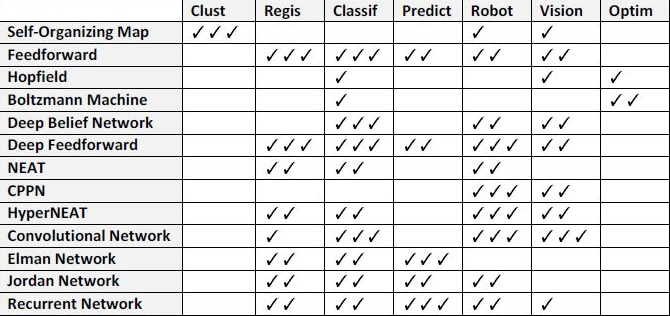
\includegraphics[scale=0.68]{images/typen_domains.png}
	\caption{Domänen zu Typen Matrix \cite{AI3}}
	\label{fig:DomainMatrix}
\end{figure}

Wie in der Abbildung \ref{fig:DomainMatrix} erkennbar ist, existiert kein Netzwerk Grundtyp, der für alle Problemdomänen geeignet ist.
Dies führt zu der Schlussfolgerung, dass je nach Aufgabe und Ziel ein entsprechendes Grundgerüst gewählt werden muss. 
Auf Basis dieses Grundgerüsts können uneingeschränkt weitere Eigenheiten aus anderen Netzwerken eingebaut werden.
In der Praxis findet man selten ein Netzwerk von einem Typ.
Meistens sind es einige mehrere Netzwerke unterschiedlicher Typen, die hintereinander und parallel geschalten sind und so ein ganzen System darstellen.
Dabei übernimmt jedes Teilnetzwerk eine kleine Aufgabe des gesamten und zwar eine für die es entwickelt wurde.
Aktuelle Netzwerke wie das Inception v3 Netzwerk von Google Research benötigt zwei Wochen mit acht Grafikkarten zum Trainieren. 
Ab diesem Zeitpunkt ist es im Stande akkurate Resultate zu liefern. 
Dieses Netzwerk ist sehr komplex und besteht nicht nur aus 3 Ebenen, was zur Schlussfolgerung führt, dass umso tiefer das Netzwerk ist, umso aufwändiger ist es zu Trainieren.

\section{Optimierung}

Optimierungen beinflussen das Lernverhalten und das Speicherverhalten eines Netzwerkes.

%Gegenmaßnahme -> dropout, Regulatoren 1/2, learnrate, momentum
\paragraph{Lernrate} skaliert die Lerngeschwindigkeit. 
Wie im Punkt Backpropagation \ref{sec:Backpropagation} beschrieben.

\paragraph{Momentum} gehört auch zur Optimierung im Algorithmus zur Backpropagation.
Dieser bestimmt wie stark frühere Gewichtsaktualisierungen berücksichtigt werden sollen. 

\paragraph{DropOut} gehört zur Kategorie der Regulatoren. 
Hinten (2012) beschreibt DropOuts als eine effektive Art, um Overfitting (siehe \ref{sec:AllgeProb}) zu vermeiden.
DropOut kann als System integriert werden, aber auch als eigener Layer in einem Netzwerk.
In einem DropOutlayer werden immer Neuronen deaktiviert, inklusive ihrer Verbindungen zu dem nächsten Layer.
Dies hat zur Folge, dass nur ein geringerer Teil an Informationen aus dem vorhergehenden Layer in den Nächsten übergeht. 
Durch diesen Prozess, des künstlichen Geringhaltens von Informationen während dem Training führt dazu, dass das Netzwerk trotz dieser Einschränkung versucht ein gutes Ergebnis zu erzielen. 
Während der Test- und Produktivphase werden diese DropOutlayer aber meist deaktiviert, da das volle Potenzial des Netzwerks verwendet werden möchte.

\paragraph{L1 und L2 Regularisierung} sind auch Techniken, die zur Verhinderung von Overfitting beitragen.
Im Gegensatz zu der DropOut Strategie sind diese zwei Regulationstechniken Teil der Backpropagation oder Teil einer Funktion.
Beide Techniken arbeiten mit Strafen, welche verteilt werden und so die Gewichtungen in ein Muster zwingen. 
%TODO objective functions -> simulated annealing
Im Falle von L1 ähnelt dieses Muster einer Gaussian Glockenkurve und bei L2 einer Laplace Kurve.
Durch das Bestrafen der Gewichtungen im Netzwerk werden diese Werte gering gehalten, sodass sie nicht ausarten. 
Wenn ein Gewicht Richtung $0$ geht, führt dies unweigerlich zu einem indirekten Ausschluss aus dem Netzwerk.
Das Netzwerk wird spärlicher und leichtgewichtiger, was aber wiederum als Resultat hat, dass ein Rauschen in den Daten möglicherweise erkannt wird und ignoriert wird.

\begin{equation}
	E := \frac{\lambda}{n} \sum\limits_{w}|w|
	\label{eq:L1ErrorTerm}
\end{equation}

Die Funktion \ref{eq:L1ErrorTerm} bildet die Berechnung der Strafe in der Backpropagation ab.
Das $\lambda$ definiert wie stark die Regulierung den Error-Wert des Netzwerkes beeinflussen soll.
Ein Wert von $0$ führt dazu, dass die Regulierung keinen Einfluss besitzt. 
Im einem normalen Fall ist dieser Wert kleiner als $0.1 (10\%)$.
Der Divisor n wird durch die Anzahl an Elementen im Trainingssatz und der Anzahl an Neuronen im Outputlayer bestimmt.
Zum Beispiel bei $100$ Elementen im Trainingssatz und $3$ Neuronen im Outputlayer würde der Divisor den Wert $300$ einnehmen.
Dies ist erforderlich da diese Funktion bei jeder Evaluierung der Trainingsdaten berechnet wird.

\paragraph{GPU - GPGPU} ist die Bezeichnung für die Verwendung des Grafikprozessors über seine ursprüngliche Auslegung darüber hinaus.
In der aktuellen Zeit ist es nicht mehr möglich eine Geschwindigkeitssteigerung zu erreichen, in dem die Taktrate des Prozessors erhöht wird. 
Deshalb wird mehr parallelisiert, da die Recheneinheiten kleiner werden und so mehrere auf der selben Fläche platz finden. 
Eine Grafikkarte besitzt die Eigenschaft, gleichförmige Operation in einem Schritt auf sehr viele Objekte gleichzeitig auszuführen. 
So werden viele Pixel in einmal eingefärbt oder eine Multiplikation großer Matrizen. 
Der Geschwindigkeitsvorteil kommt dabei durch den hohen Grad an Parallelität, da die Grafikkarte hauptsächlich für solche Operationen ausgelegt worden ist.

\paragraph{Batch Learning} gehört nicht direkt in die Kategorie der Optimierung, bietet trotzdem einen Performanzvorteil. 
Durch Batch Learning wird immer ein Paket in das System eingeführt. 
Dieses Paket wird je nach Implementierung parallel verarbeitet oder sequenziell. 
Der Unterschied zu 'Online Learning' ist nun, dass nicht nach jedem Durchlauf die Gewichtungen und das System nachjustiert werden, sondern dass zu Erst das Paket verarbeitet wird und das System einmal angepasst wird. 
Wenn also ein Paket mit einer Größe von $64$ in das System eingeführt wird, führt dies einmal zu einer Anpassung des Graphen, in dem die Gradienten zusammen gerechnet werden und einmal auf den Graphen adaptiert werden. \cite{AI3}

%\section{Tensorflow Typen Unterstützung}





